\section{Approach \& Uniqueness}

In order to enforce reservations while still running best effort jobs
opportunistically, our approach is use priority scheduling.

Enforcing priorities requires fewer global runqueue searches than weights do,
because they only need to happen on \textit{class boundary crossings}: on
\exit{}, when a core switches to running lower class processes after having
previously been running high class, and on \entry{}, when a core enqueues a
higher class process. These checks ensure that a core $c$ running a BE thread
$t$ knows that there are no queued LC threads anywhere on the machine. If there
was one when $c$ starts running $t$, the \exit{} check would see and steal it.
If a new LC thread wakes up on a different core while $t$ is running, the
\entry{} check ensures that core will look at $c$'s runqueue and run the new LC
thead on $c$, interrupting $t$.

\begin{figure}[t]
    \centering
    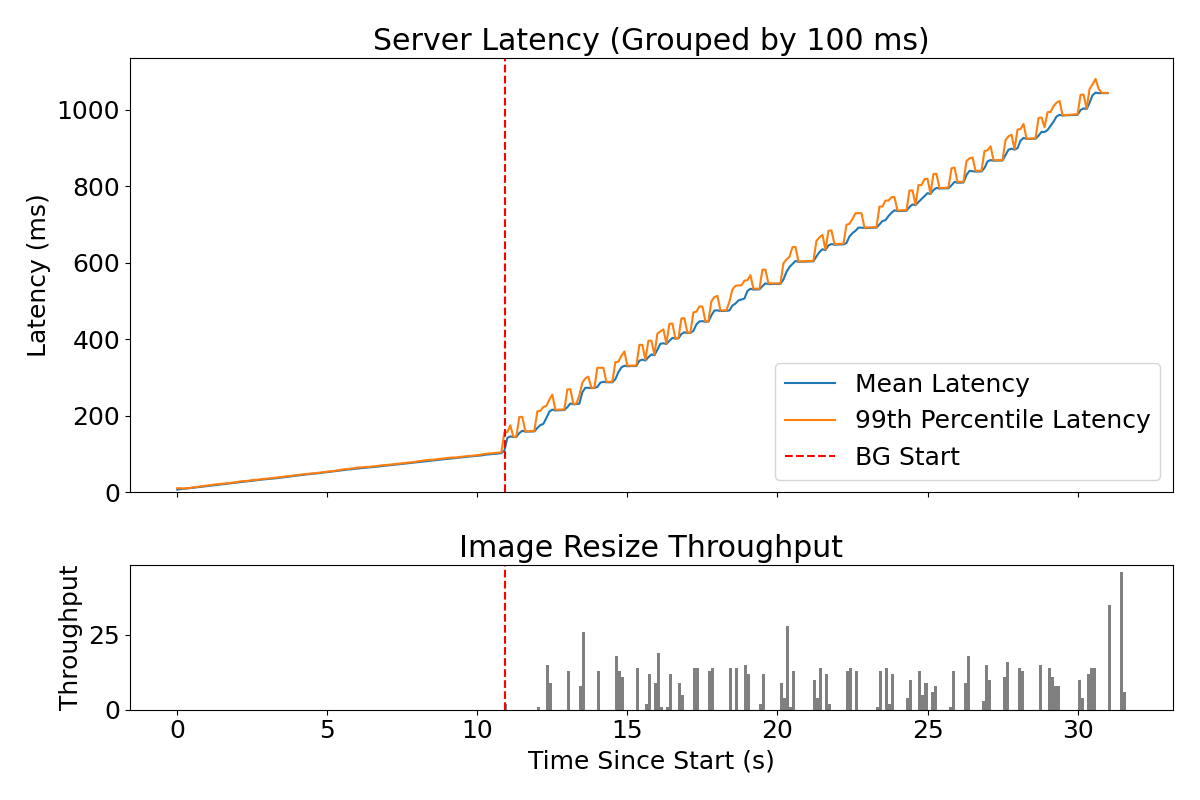
\includegraphics[width=\columnwidth]{graphs/overload-rt.png}
    \caption{LC in real time, throttling}\label{fig:overload-rt}
\end{figure}


Linux already provides priority scheduling across scheduling classes, which are
used to separate real-time applications from all other workloads. However, the
scheduling algorithm used for real-time applications differs from the one for
the default class. Additionally, the priority between real-time and the default
scheduling classes comes with an asterisk: if real-time applications experience
high load, Linux throttles them in order to not starve the default class. We can
see this happening in \autoref{fig:overload-rt}, where throttling leads to
spikes in the background task as it is able to run, and corresponding spikes in
the server's latency.

We design a new scheduling class \beclass{} that sits at a lower priority than
\normalclass{}, which enforces LC applications' uncontended access to the CPUs
they reserved. To enforce reservations even under high load, without throttling
the latency critical services or killing the BE ones, \beclass{} \textit{parks}
BE processes meaning the user-space code never runs, only kernel-level
services.